%%
%% Felex manuscript — Russian internal review version
%% Format: cas-sc (matching EN submission layout exactly)
%% Compile with: xelatex + bibtex
%%

\documentclass[a4paper,fleqn]{cas-sc}

% XeLaTeX font and language support
\usepackage{fontspec}
\defaultfontfeatures{Ligatures=TeX}
\usepackage{polyglossia}
\setmainlanguage{russian}
\setotherlanguage{english}
\setmainfont{Times New Roman}
\newfontfamily\cyrillicfont{Times New Roman}

\usepackage[authoryear]{natbib}

% Algorithm support
\usepackage{algorithm}
\usepackage{algpseudocode}

\begin{document}
\let\WriteBookmarks\relax
\def\floatpagepagefraction{1}
\def\textpagefraction{.001}

% Short title (for running head)
\shorttitle{Felex: локальная платформа для рационов}

% Short author list (for running head)
\shortauthors{Д.Д. Котельников и О.В. Демкина}

% Main title of the paper
\title[mode=title]{Felex: локальная платформа поддержки принятия решений для составления рационов в малых хозяйствах и животноводческом бизнесе России}

% Title footnote
\tnotemark[1]
\tnotetext[1]{Рукопись подана для публикации в Livestock Science (Elsevier). Данная версия подготовлена для внутреннего рецензирования.}

% First author - Danil D. Kotelnikov
\author[1]{Данил Д. Котельников}[orcid=0009-0003-5159-5796]
\ead{danil.kotelnikov.02@mail.ru}
\ead[url]{https://github.com/danilkotelnikov/Felex}
\credit{Методология, Программное обеспечение, Подготовка данных, Формальный анализ, Исследование, Написание — рецензирование и редактирование, Визуализация, Валидация, Ресурсы, Научное руководство, Администрирование проекта}
\affiliation[1]{organization={Дальневосточный государственный аграрный университет},
                addressline={ул. Политехническая, 86},
                city={Благовещенск},
                postcode={675005},
                state={Амурская область},
                country={Россия}}

% Second author - Olga V. Demkina (Corresponding)
\author[1]{Ольга В. Демкина}[orcid=0000-0001-9303-4100]
\cormark[1]
\ead{demkina1976@gmail.com}
\credit{Концептуализация, Написание — подготовка исходной версии}
\affiliation[1]{organization={Дальневосточный государственный аграрный университет},
                addressline={ул. Политехническая, 86},
                city={Благовещенск},
                postcode={675005},
                state={Амурская область},
                country={Россия}}

% Corresponding author text
\cortext[cor1]{Автор для корреспонденции: demkina1976@gmail.com}

% Abstract (structured per Livestock Science requirements — 6 headings)
\begin{abstract}
\textbf{Цель и актуальность:} Математическая формализация рационов остается одной из ключевых задач цифровой поддержки решений в животноводстве. Для малых хозяйств и животноводческого бизнеса России выбор программного обеспечения ограничен региональными кормовыми базами, необходимостью совмещения отечественных и международных нормативов, периодическими проблемами со связью и низкой терпимостью к непрозрачным облачным сервисам. Система Felex разработана как гибридное настольное приложение (Rust--React--Tauri), реализующее прозрачные рабочие процессы линейного программирования для расчета рационов с локальным агентным контуром для ограниченной интерпретации результатов.

\textbf{Сбор данных:} Нормализованный исходный экспорт кормовой базы содержал 2723 записи. Готовый к benchmark каталог включал 1342 оценённые по стоимости кормовые позиции, собранные из 151 прямого ценового якоря и 1191 benchmark-цены, полученной через fallback-пайплайн.

\textbf{Методы исследования:} Оптимизационный benchmark включал 23 животноводческих сценария по трём рабочим процессам (\texttt{build\_from\_library}, \texttt{complete\_from\_library}, \texttt{selected\_only}), что составило 69 запусков. Две конфигурации Qwen 3.5 (4B/4096 и 9B/2048) были протестированы как ограниченные консультанты на 12 задачах с отключённым web search; benchmark-телеметрия фиксировала effective model/context и fallback-статус.

\textbf{Результаты:} По всем оптимизационным запускам среднее время расчёта составило 246{,}6~мс, средняя доля выполненных жёстких ограничений~--- 64{,}8\%, средний индекс покрытия норм~--- 81{,}8/100. Наилучшее покрытие показал рабочий процесс \texttt{complete\_from\_library} (85{,}0), тогда как \texttt{selected\_only} оказался самым быстрым (0{,}41~мс). Обе конфигурации агента показали одинаковый результат (общая применимость 34{,}2/100) без скрытого fallback.

\textbf{Заключение:} Felex демонстрирует, что локально развертываемая платформа для расчёта рационов может сочетать прозрачную оптимизацию, поддержку нескольких нормативных контуров и практичную настольную среду выполнения без привязки к cloud-first архитектуре.

\textbf{Вклад:} Основными преимуществами являются локальное развертывание и явные рабочие процессы; текущие ограничения связаны с покрытием кормовой базы, линейной моделью оптимизации и недостаточной надежностью агента для полноценного консультирования.
\end{abstract}

% Graphical abstract omitted — no repository-backed asset present
% in the audited submission bundle.

% Research highlights (3-5 bullets, max 85 characters each)
\begin{highlights}
\item Локальная система поддержки решений по рационам для малых хозяйств России
\item Три рабочих процесса оценены на 23 сценариях и 69 запусках
\item complete\_from\_library показал наилучшее среднее покрытие норм (85{,}0)
\item Среднее время оптимизации составило 246{,}6 мс по всем процессам
\item Локальные агенты 4B и 9B непригодны для надежного консультирования
\end{highlights}

% Keywords (1-7 terms, separated by \sep)
\begin{keywords}
кормление животных \sep составление рационов \sep поддержка решений \sep линейное программирование \sep настольное ПО \sep Россия
\end{keywords}

\maketitle

% Main text
\section{Введение}\label{sec:introduction}

Математическая формализация рационов остается одной из ключевых задач цифровой поддержки решений в животноводстве, поскольку при построении рациона необходимо одновременно учитывать биологические потребности животных, наличие кормов и экономические ограничения \citep{nASEM2021, dantzig1963, zhai2020, tedeschi2021smart}. Современный рынок программных продуктов для этих задач уже сформирован и включает как крупные формуляционные комплексы, так и более узкие инструменты для консультантов и хозяйств \citep{datacor2026, mixit2026, winfeed2026, korall2026, deltakorm2026, onecow2026, winmix2026}. Следовательно, речь идет не о заполнении пустой ниши, а о корректном позиционировании нового инструмента внутри неоднородного программного поля. Англоязычные и американские решения демонстрируют более высокую коммерческую зрелость и интеграцию с корпоративными контурами, тогда как российские продукты, как правило, лучше адаптированы к локальной практике, но остаются закрытыми и вендор-зависимыми.

Для малых хозяйств и животноводческого бизнеса России к этому добавляются специфические ограничения: региональная неоднородность кормовых баз, необходимость сочетать отечественные и международные нормы, периодические проблемы со связью и низкая терпимость к непрозрачным облачным сервисам \citep{kalashnikov2003, vizh2020, aquilani2022, selvaggi2024}. В таких условиях практическую ценность имеет не тот инструмент, который пытается заменить всю существующую цифровую экосистему, а тот, который обеспечивает локальную прозрачную оптимизацию, воспроизводимую логику нормирования и понятный специалисту рабочий процесс.

Система Felex была разработана именно для этой более узкой прикладной ниши. Это гибридное настольное приложение (Rust--React--Tauri), реализующее рабочие процессы линейного программирования для расчёта рационов и включающее локальный агентный контур для интерпретации результатов. Цель настоящей работы~--- описать текущую исполняемую архитектуру системы, представить результаты benchmark-оценки оптимизационного ядра и определить, в какой мере существующий локальный агент пригоден для вспомогательной интерпретации рассчитанных рационов в практическом животноводческом контуре.

\section{Материалы и методы}\label{sec:methods}

\subsection{Архитектура системы}\label{subsec:architecture}

Felex реализует многоуровневую архитектуру, разделяющую пользовательский интерфейс, вычислительный контур и слой данных. Клиентская часть построена на React~18 и TypeScript с использованием Zustand для управления состоянием. Оптимизационный бэкенд написан на Rust \citep{rust2023} и использует библиотеку \texttt{good\_lp} \citep{goodlp2023} для решения задач линейного программирования. Настольная упаковка обеспечивается фреймворком Tauri \citep{tauri2023}, однако фактический runtime не сводится к чистому Tauri IPC: настольная оболочка запускает встроенный локальный HTTP-бэкенд, а frontend взаимодействует с оптимизатором через тот же API-контур, который используется и в режиме локальной браузерной разработки. Локальный слой данных опирается на SQLite и сгенерированные JSON-артефакты.

Агентный слой по умолчанию работает через Ollama, но в кодовой базе также реализована поддержка OpenAI-совместимых интерфейсов. В текущем benchmark агент рассматривался как ограниченный консультант, а не как автономный формуляционный модуль; все агентные тесты были выполнены с отключённым web search.

Общий исполняемый контур системы показан на рисунке~\ref{fig:architecture}.

\begin{figure}[htbp]
    \centering
    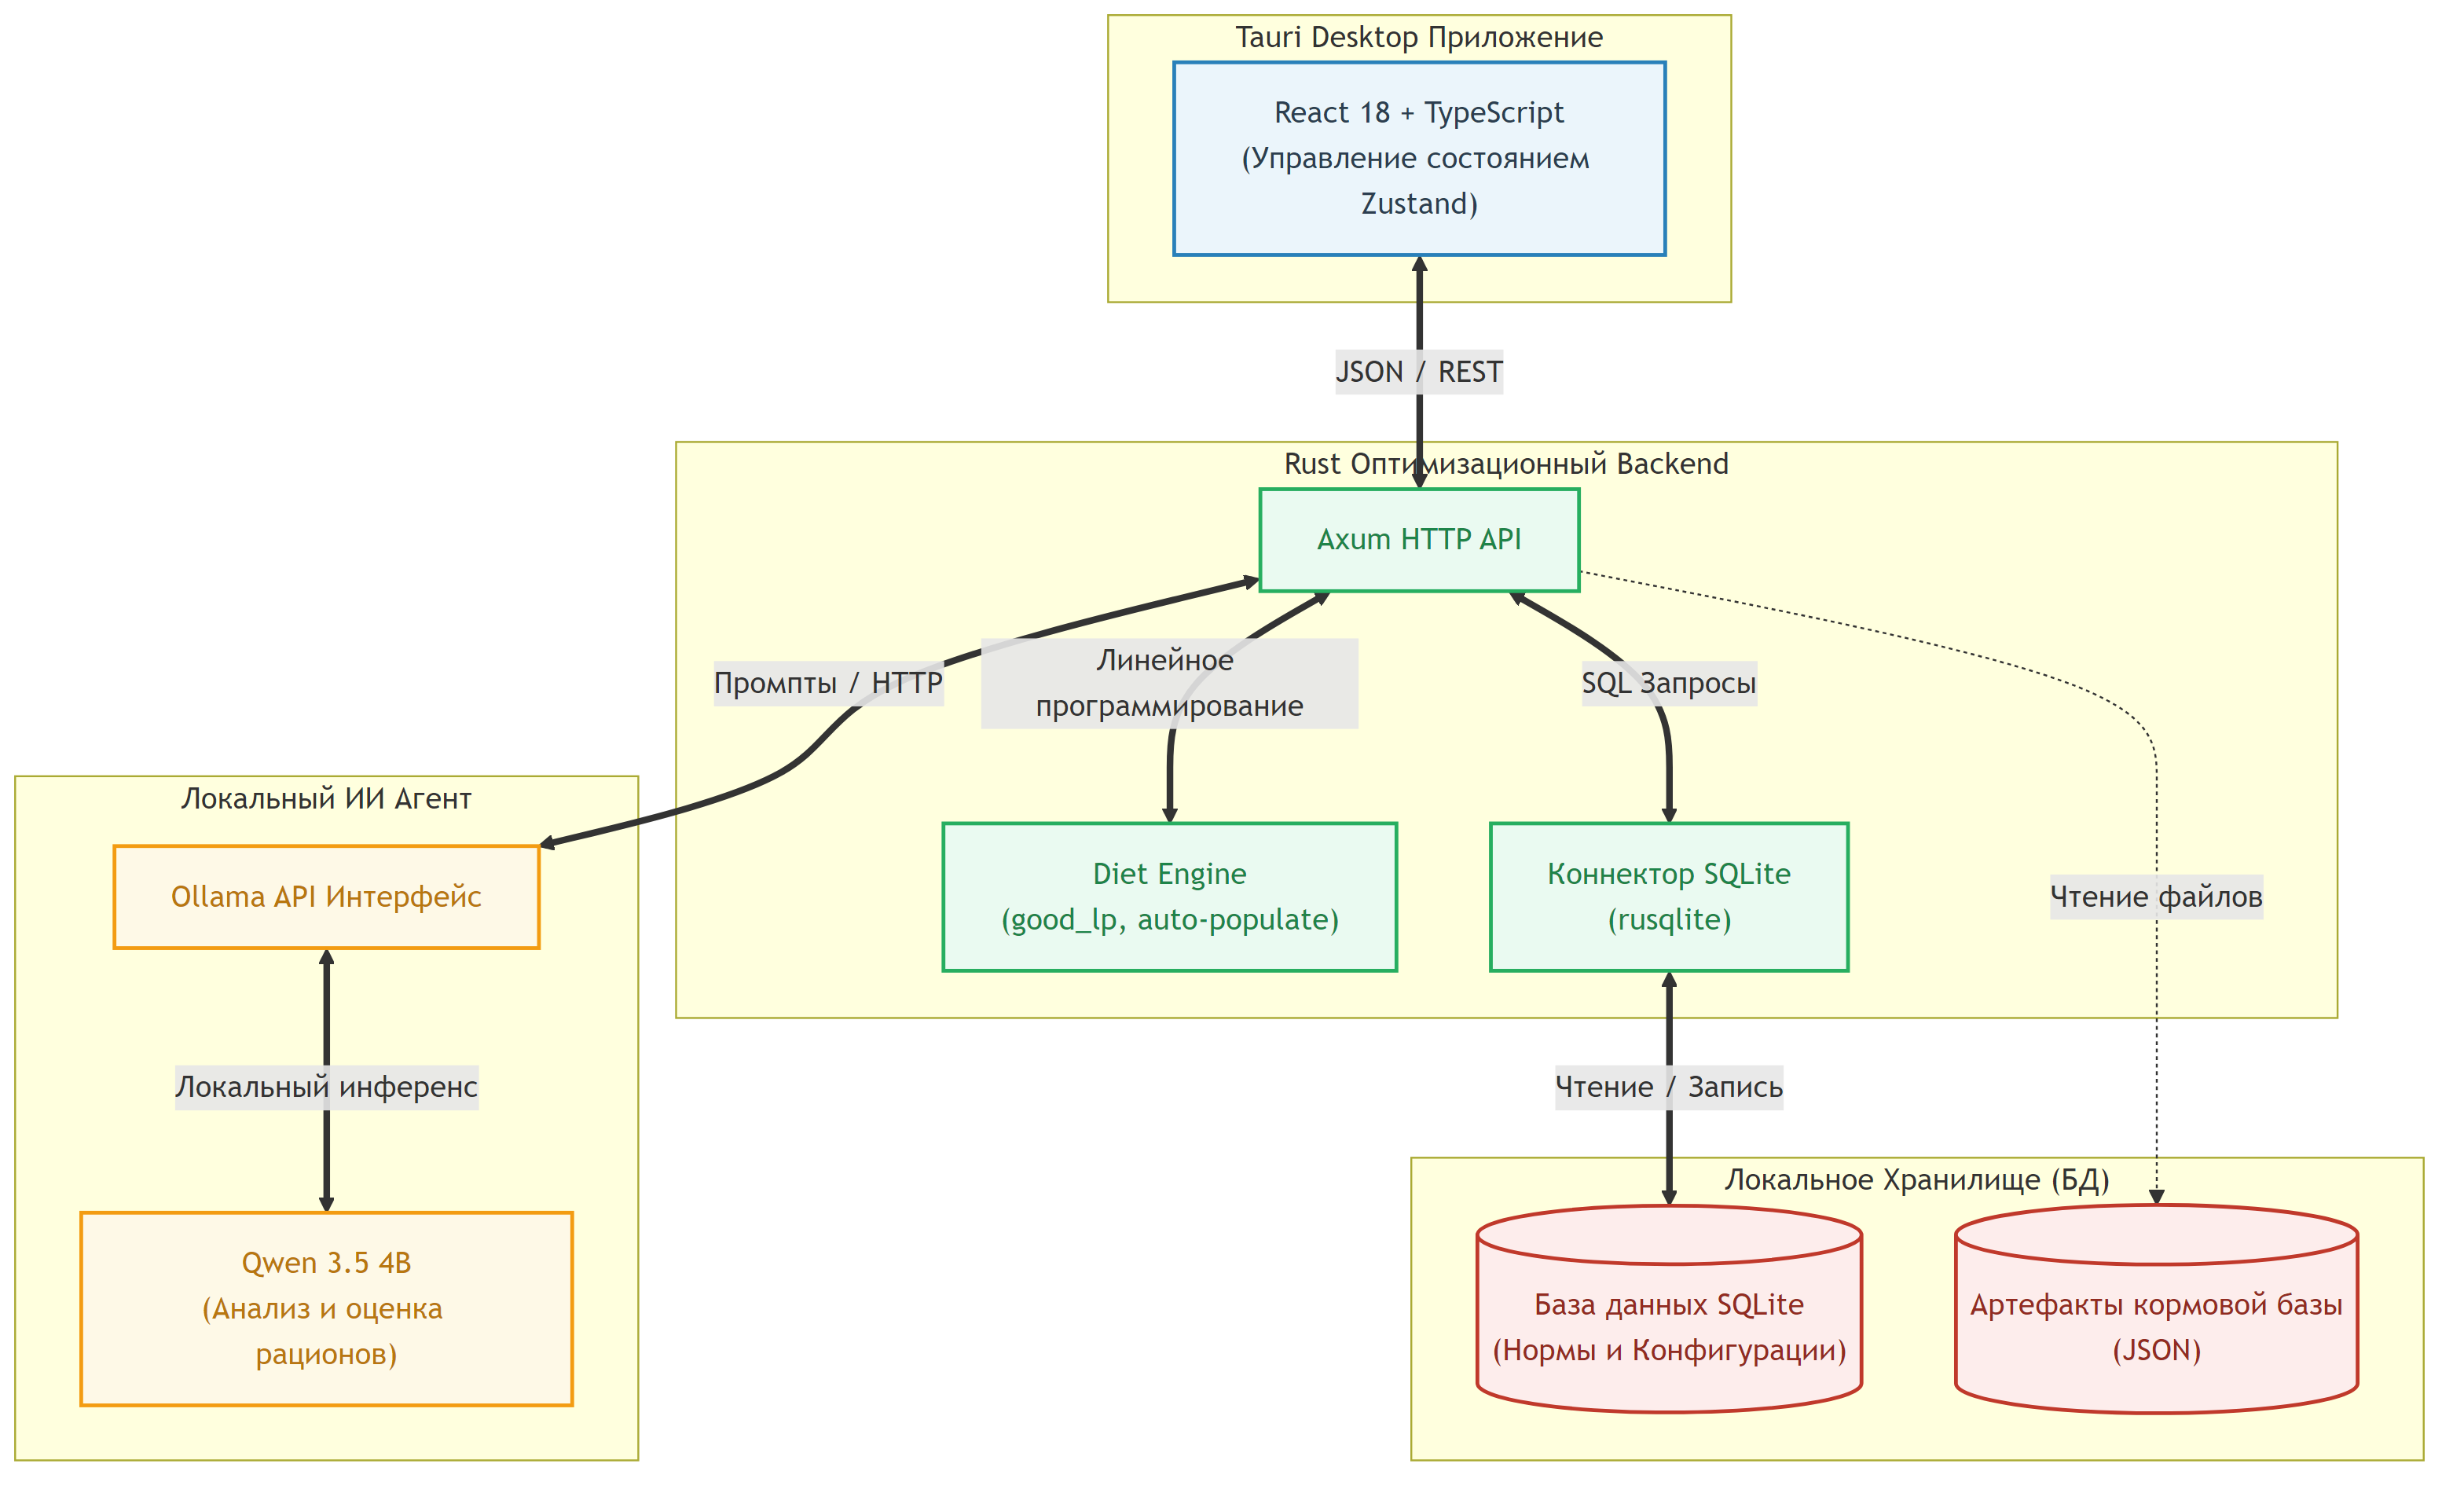
\includegraphics[width=0.95\textwidth]{figures/system_architecture_ru.png}
    \caption{Архитектура Felex, иллюстрирующая взаимодействие между пользовательским интерфейсом на React, встроенным Rust HTTP-бэкендом, локальной базой данных и локальным агентным контуром.}
    \label{fig:architecture}
\end{figure}

\subsection{Кормовая база данных и система нутриентов}\label{subsec:database}

Основой для работы алгоритма служит база данных кормов, полученная путем автоматизированного извлечения и систематизации информации из открытого справочника vidkormov.narod.ru. Разработанный на Python конвейер выполняет сбор, перевод и нормализацию данных, формируя локальную SQLite-базу. Нормализованный исходный экспорт в текущем состоянии содержит 2723 кормовые записи. При этом benchmark-ready каталог, использованный в настоящем вычислительном эксперименте, включает 1342 ценово обеспеченные кормовые позиции; из них 151 имеют прямые ценовые якоря, а 1191 получили benchmark-цены через fallback-процедуру сопоставления. Библиотека охватывает грубые, сочные и концентрированные корма, белковые добавки, минеральные компоненты, премиксы, побочные продукты переработки, корма животного происхождения и источники небелкового азота (NPN).

\textbf{Цены в benchmark-каталоге являются синтетическими и используются исключительно для оценки рабочих процессов}; они не отражают реальную рыночную конъюнктуру. Нормализованный экспорт (2723 записи) представляет справочные данные без ценовой информации.

Встроенная схема базы данных (\texttt{feeds}) поддерживает расчёт по 31 ключевому нутриенту и связанным полям состава кормов, формирующим оптимизационный контур. К ним относятся сухое вещество, три видоспецифичных показателя обменной энергии (\texttt{energy\_oe\_cattle}, \texttt{energy\_oe\_pig}, \texttt{energy\_oe\_poultry}), сырой и переваримый протеин (\texttt{dig\_protein\_cattle}, \texttt{dig\_protein\_pig}, \texttt{dig\_protein\_poultry}), аминокислоты (лизин, метионин + цистин), сырой жир, сырая клетчатка, крахмал, сахар, макро- и микроэлементы (Ca, P, Mg, K, Na, S, Fe, Cu, Zn, Mn, Co, I) и витамины/предшественники (каротин, витамины D3 и E). Производные соотношения и процентные ограничения формируются внутри оптимизатора на основе этих хранимых полей.

Использование видоспецифичных энергетических метрик обусловлено фундаментальными различиями в пищеварении. Для жвачных животных (КРС) энергетическая ценность корма оценивается по обменной энергии (\texttt{energy\_oe\_cattle}) с учётом процессов рубцового брожения, что концептуально согласуется с современными моделями оценки питательности \citep{sauvant2018, nASEM2021}. Для моногастричных животных используются метрики \texttt{energy\_oe\_pig} и \texttt{energy\_oe\_poultry}. Единицы измерения норм также различаются: для КРС преобладают абсолютные суточные значения (МДж и граммы в сутки), тогда как для свиней и птицы чаще используются относительные концентрации (г/кг корма или проценты рациона).

Важная особенность системы для моногастричных животных~--- учёт переваримости при нормировании аминокислотных ограничений. Текущая реализация интерпретирует требования к стандартизированной илеальной переваримости (SID) и истинной илеальной переваримости (TID) через нормативный и оптимизационный слой с обработкой псевдонимов/fallback при отсутствии разделённых полей профиля корма. Переход от оценки общего содержания аминокислот к илеально-переваримым формам является общепринятым международным стандартом \citep{stein2007, nRC2012, nRC1994}, поскольку позволяет точнее характеризовать биологическую доступность белка и уменьшать избыточную азотную нагрузку \citep{pomar2021, deLange2012, vanmilgen2015}.

Для экономической оценки benchmark движок сначала импортирует актуальные неинферированные ценовые якоря из рабочей базы данных Felex, а затем заполняет оставшийся benchmark-каталог через явный fallback-пайплайн по подкатегории, категории, семейству и глобальным медианам. Это формирует полностью оценённый benchmark-каталог с сохранением меток происхождения прямых и инферированных цен.

\subsection{Нормы кормления и их производные}\label{subsec:norms}

Система реализует многоуровневый процесс расчёта зоотехнических норм: от базовых значений в таблицах базы данных до видоспецифичных динамических моделей и факториальных расчётов. Для обеспечения максимальной точности к нормам применяются механизмы контекстного масштабирования в зависимости от физиологического состояния животного (живая масса, продуктивность, возраст, пол).

Для лактирующих коров применяется динамическая модель оценки потребления сухого вещества (DMI) и чистой энергии лактации (NEL). Энергетические потребности складываются из поддерживающего метаболизма, зависящего от метаболической массы тела ($BW^{0{,}75}$), и лактационных затрат, рассчитанных на основе 4\%-ного жирокорригированного молока (FCM). Базовые уравнения и породные поправочные коэффициенты адаптированы из классических методик \citep{nRC2001, kalashnikov2003}.

Для свиней на откорме используется билинейная интерполяция нормативных таблиц по живой массе и среднесуточному приросту. Модель динамически рассчитывает потребности в обменной энергии, протеине и стандартизированных илеально-переваримых аминокислотах, масштабируя их в зависимости от ожидаемой интенсивности роста \citep{nRC2012}.

Учёт кормления птицы ведётся по фазам. Для бройлеров потребности в аминокислотах (TID-лизин, TID-метионин+цистин) задаются как строгие проценты рациона в зависимости от периода выращивания (стартер, гроувер, финишер) \citep{vnitip2017, nRC1994}. Для кур-несушек используется факториальный подход к расчёту кальция, суммирующий потребности на поддержание жизни и затраты на формирование скорлупы в зависимости от уровня яйценоскости.

Вычислительное ядро основано на программном факториальном фреймворке (\texttt{NutrientCalculator}), суммирующем компоненты потребностей (поддержание, рост, продукция, лактация, супоросность) с учётом коэффициентов усвоения. Различия в единицах измерения норм являются принципиальными: жвачные потребляют большие объёмы грубых кормов переменного состава, поэтому баланс поддерживается в абсолютных суточных количествах на голову, тогда как моногастричные животные получают полнорационные комбикорма со строго контролируемыми концентрациями нутриентов (проценты или г/кг).

\subsection{Структурная матрица кормов}\label{subsec:matrix}

Для обеспечения биологической адекватности рациона, помимо нутриентного баланса, необходимо соблюдать структурные пропорции. С этой целью в оптимизатор интегрирована матрица кормов, задающая допустимые границы (минимум, оптимум, максимум в процентах от сухого вещества) для различных категорий кормов.

Система автоматически классифицирует каждый ингредиент (\texttt{classify\_feed}), относя его к одной из функциональных групп: грубые, концентрированные, сочные, минеральные корма, премиксы, корма животного происхождения или источники небелкового азота (NPN). На основе этих категорий накладываются видоспецифичные структурные ограничения. Например, для поддержания нормальной физиологии рубца у молочного КРС доля грубых кормов должна составлять от 35\% до 65\% сухого вещества, тогда как рационы бройлеров состоят почти исключительно из концентратов.

Исключение из строгих правил матрицы делается для отдельных физиологических групп, таких как супоросные свиноматки, рацион которых формируется преимущественно на основе индивидуальных ограничений по включению конкретных ингредиентов и целевой калорийности. Помимо матричных пропорций, движок поддерживает индивидуальные ограничения на максимальный процент включения отдельных кормов (например, строгий контроль включения мочевины или высокожирных кормов).

\subsection{Математическая модель оптимизационного ядра и рабочие процессы}\label{subsec:optimization}

Движок Felex формулирует задачу построения рациона как задачу линейного программирования с иерархическими ограничениями (tiered constraints). Пусть $x \in \mathbb{R}^n$~--- вектор количеств используемых кормов (в кг натуральной или сухой массы), где $n$~--- общее число доступных ингредиентов. Вектор стоимостей кормов обозначим $c \in \mathbb{R}^n$. Целевая функция минимизирует общую стоимость рациона:
\begin{equation}
\min_{x} \quad z = c^T x
\end{equation}

Ограничения задаются матрицей питательных веществ $A \in \mathbb{R}^{m \times n}$ и векторами минимальных $b_{\min} \in \mathbb{R}^m$ и максимальных $b_{\max} \in \mathbb{R}^m$ требований:
\begin{equation}
b_{\min} \leq A x \leq b_{\max}, \quad x \geq 0
\end{equation}

Для обеспечения разрешимости задачи при конфликтующих требованиях применяется аддитивная иерархия ограничений. Абсолютные пределы (например, максимальное потребление сухого вещества, структурная матрица кормов) накладываются как нерелаксируемые LP-ограничения вне уровневой системы. Нутриентные ограничения разделены на три уровня:
\begin{itemize}
    \item \textbf{Уровень 1}: Ключевые (жёсткие) нутриенты (обменная энергия, сырой протеин, кальций, фосфор).
    \item \textbf{Уровень 2}: Стандартные нутриенты (лизин, метионин, сырая клетчатка). Система поддерживает механизмы fallback: например, при отсутствии стандартизированного илеально-переваримого лизина (\texttt{lysine\_sid}) в профиле корма используется общее значение \texttt{lysine}.
    \item \textbf{Уровень 3}: Мягкие ограничения~--- микроэлементы и витамины (цинк, медь, витамины E и D3).
\end{itemize}

Оптимизатор реализует три концептуальных рабочих процесса:
\begin{enumerate}
    \item \texttt{build\_from\_library}: Автоматическое построение (неограниченный поиск). Структурная матрица кормов применяется для соблюдения допустимых категориальных пропорций (напр., <<грубые $\geq 40\%$ СВ>>).
    \item \texttt{complete\_from\_library}: Балансировка пользовательского <<каркаса>> рациона. Пользовательские ограничения по конкретным ингредиентам фиксируются, недостающие нутриенты покрываются из библиотеки.
    \item \texttt{selected\_only}: Ограниченный поиск исключительно в заранее выбранном пользователем наборе кормов без возможности введения новых ингредиентов.
\end{enumerate}

Рабочий процесс оптимизатора (Алгоритм~\ref{alg:optimizer}) использует метод аддитивного построения ограничений, фиксируя достигнутые целевые уровни с предыдущего уровня. В случае нерешимости строгой уровневой задачи применяется механизм целевого программирования (мягкие цели со штрафными функциями).

\begin{algorithm}[htbp]
\caption{Аддитивный иерархический алгоритм оптимизации рационов (Diet Engine)}\label{alg:optimizer}
\begin{algorithmic}[1]
\Require Вектор стоимостей $c$, матрица нутриентов $A$, векторы потребностей $b_{\min}, b_{\max}$, набор доступных кормов $F$.
\Ensure Оптимальный вектор $x^*$.
\State $T \gets \emptyset$ \Comment{Текущий набор ограничений (помимо базовых пределов потребления)}
\State $B \gets \emptyset$ \Comment{Зафиксированные целевые полосы для ранее достигнутых нутриентов}
\For{$L \in \{\text{Уровень 1}, \text{Уровень 2}, \text{Уровень 3}\}$}
    \State $T \gets T \cup L$
    \State Решить LP-подзадачу: оптимизировать целевую функцию для нутриентов $T$ с учётом полос $B$.
    \If{Решение $x$ найдено}
        \State Обновить $x^* \gets x$
        \State Добавить достигнутые уровни нутриентов $L$ в полосы $B$ (с допуском).
    \Else
        \State \textbf{break}
    \EndIf
\EndFor
\If{$x^*$ не определён (нерешимость даже для Уровня~1)}
    \State $x^* \gets \text{решение методом целевого программирования (взвешенные штрафы)}$.
\Else
    \State Выполнить финальную минимизацию стоимости: $\min c^T x$ при ограничениях $B$.
\EndIf
\State \Return $x^*$ и достигнутый нутриентный профиль $A x^*$.
\end{algorithmic}
\end{algorithm}

\subsection{Методология вычислительного эксперимента и генерация артефактов}\label{subsec:experiment}

Для оценки практической производительности было проведено вычислительное тестирование с использованием канонического benchmark-артефакта, сгенерированного текущим benchmark-пайплайном Felex. Авторский каталог сценариев содержит 40 сценариев, однако исполняемый benchmark в настоящее время включает 23 реализованных животноводческих сценария (молочный и мясной КРС, свиньи, птица; дополнительная Таблица~S1). Посценарные исходы оптимизации для этих случаев представлены в дополнительной Таблице~S2. Benchmark-ready каталог содержал 1342 оценённые по стоимости кормовые позиции; из них 151 имели прямые ценовые якоря, а оставшиеся 1191 benchmark-цена были получены через fallback-пайплайн ценообразования. Для каждого реализованного сценария оптимизация выполнялась по трём рабочим процессам: \texttt{build\_from\_library}, \texttt{complete\_from\_library} и \texttt{selected\_only}, что составило 69 запусков. Результаты (время выполнения, доли выполнения ограничений, стоимости, компоненты дефицитов/избытков и индексы покрытия норм) были программно экспортированы в JSON, а затем преобразованы в производные CSV-таблицы и графические ассеты.

Все графики, таблицы и статистические сводки были программно сгенерированы из benchmark JSON для исключения ошибок ручной транскрипции данных. Для оценки общего качества результирующего рациона benchmark использовал реализованный в Felex индекс адекватности (представленный здесь как Индекс покрытия норм, шкала 0--100). Для каждого оцениваемого ограничения $k$ с фактическим значением $a_k$, нижней границей $L_k$, верхней границей $U_k$ и целевым значением $T_k$ benchmark вычислял:
\begin{equation}
 d^-_k = \max\left(0, \frac{L_k - a_k}{L_k}\right), \qquad
 d^+_k = \max\left(0, \frac{a_k - U_k}{U_k}\right), \qquad
 g_k = \frac{|a_k - T_k|}{|T_k|}
\end{equation}
Агрегированный индекс определялся как
\begin{equation}
\text{Покрытие} = \frac{100}{1 + \bar{P}}
\end{equation}
где $\bar{P}$~--- средневзвешенное по уровням значение $d^-_k + d^+_k + 0{,}25 g_k$ по контролируемому множеству ограничений с использованием реализованных в Felex приоритетных весов (Уровень~1 = 3, Уровень~2 = 2, Уровень~3 = 1). Дельта качества (Quality Delta) вычислялась как разность этого индекса между процессами \texttt{complete\_from\_library} и \texttt{build\_from\_library}.

Локальный агентный слой оценивался как ограниченный консультационный помощник через нативный агентный стек Felex, а не через прямые запросы к Ollama. Все агентные тесты выполнялись последовательно с отключённым web search для снижения неконтролируемой латентности. Две локальные конфигурации были протестированы: Qwen 3.5 4B при 4096 токенах контекста и Qwen 3.5 9B при 2048 токенах контекста \citep{qwen2023, ollama2023}. Benchmark включал шесть задач диагностики рационов на основе разреженных стартовых рационов и шесть задач поиска кормов, привязанных к benchmark-каталогу. Метрики включали recall лимитирующих нутриентов@3, overlap рекомендаций@3, обоснованность рекомендаций@3, точность lookup и общий балл применимости, определяемый как $100 \times (0{,}45 \times \text{recall} + 0{,}25 \times \text{groundedness} + 0{,}10 \times \text{overlap} + 0{,}20 \times \text{lookup accuracy})$. Benchmark-телеметрия также фиксировала effective model, effective context window и наличие скрытого fallback при выполнении каждой задачи. Данная оценка была направлена на определение ограниченной вспомогательной пригодности, а не готовности к автономному консультированию.

\section{Результаты}\label{sec:results}

\subsection{Вычислительная производительность}\label{subsec:performance}

Анализ 69 запусков выявил выраженные структурные различия в производительности между рабочими процессами (Рисунок~\ref{fig:runtime}). Среднее время выполнения по всей выборке составило 246{,}6~мс. Наиболее ресурсоёмким оказался процесс \texttt{build\_from\_library} со средним временем 617{,}5~мс, что закономерно связано с поиском по наиболее широкому пространству ингредиентов под ограничениями матрицы и норм. Процесс \texttt{complete\_from\_library} занимал в среднем 121{,}8~мс, тогда как строго ограниченный \texttt{selected\_only} выполнялся в среднем за 0{,}41~мс. Агрегированные показатели по рабочим процессам сведены в дополнительной Таблице~S3, а видоспецифичные benchmark-сводки, используемые далее при экономической интерпретации~--- в дополнительной Таблице~S4. В текущем benchmark все три рабочих процесса остаются операционно интерактивными, а основной компромисс определяется шириной поиска, а не неприемлемой задержкой.

\begin{figure}[htbp]
    \centering
    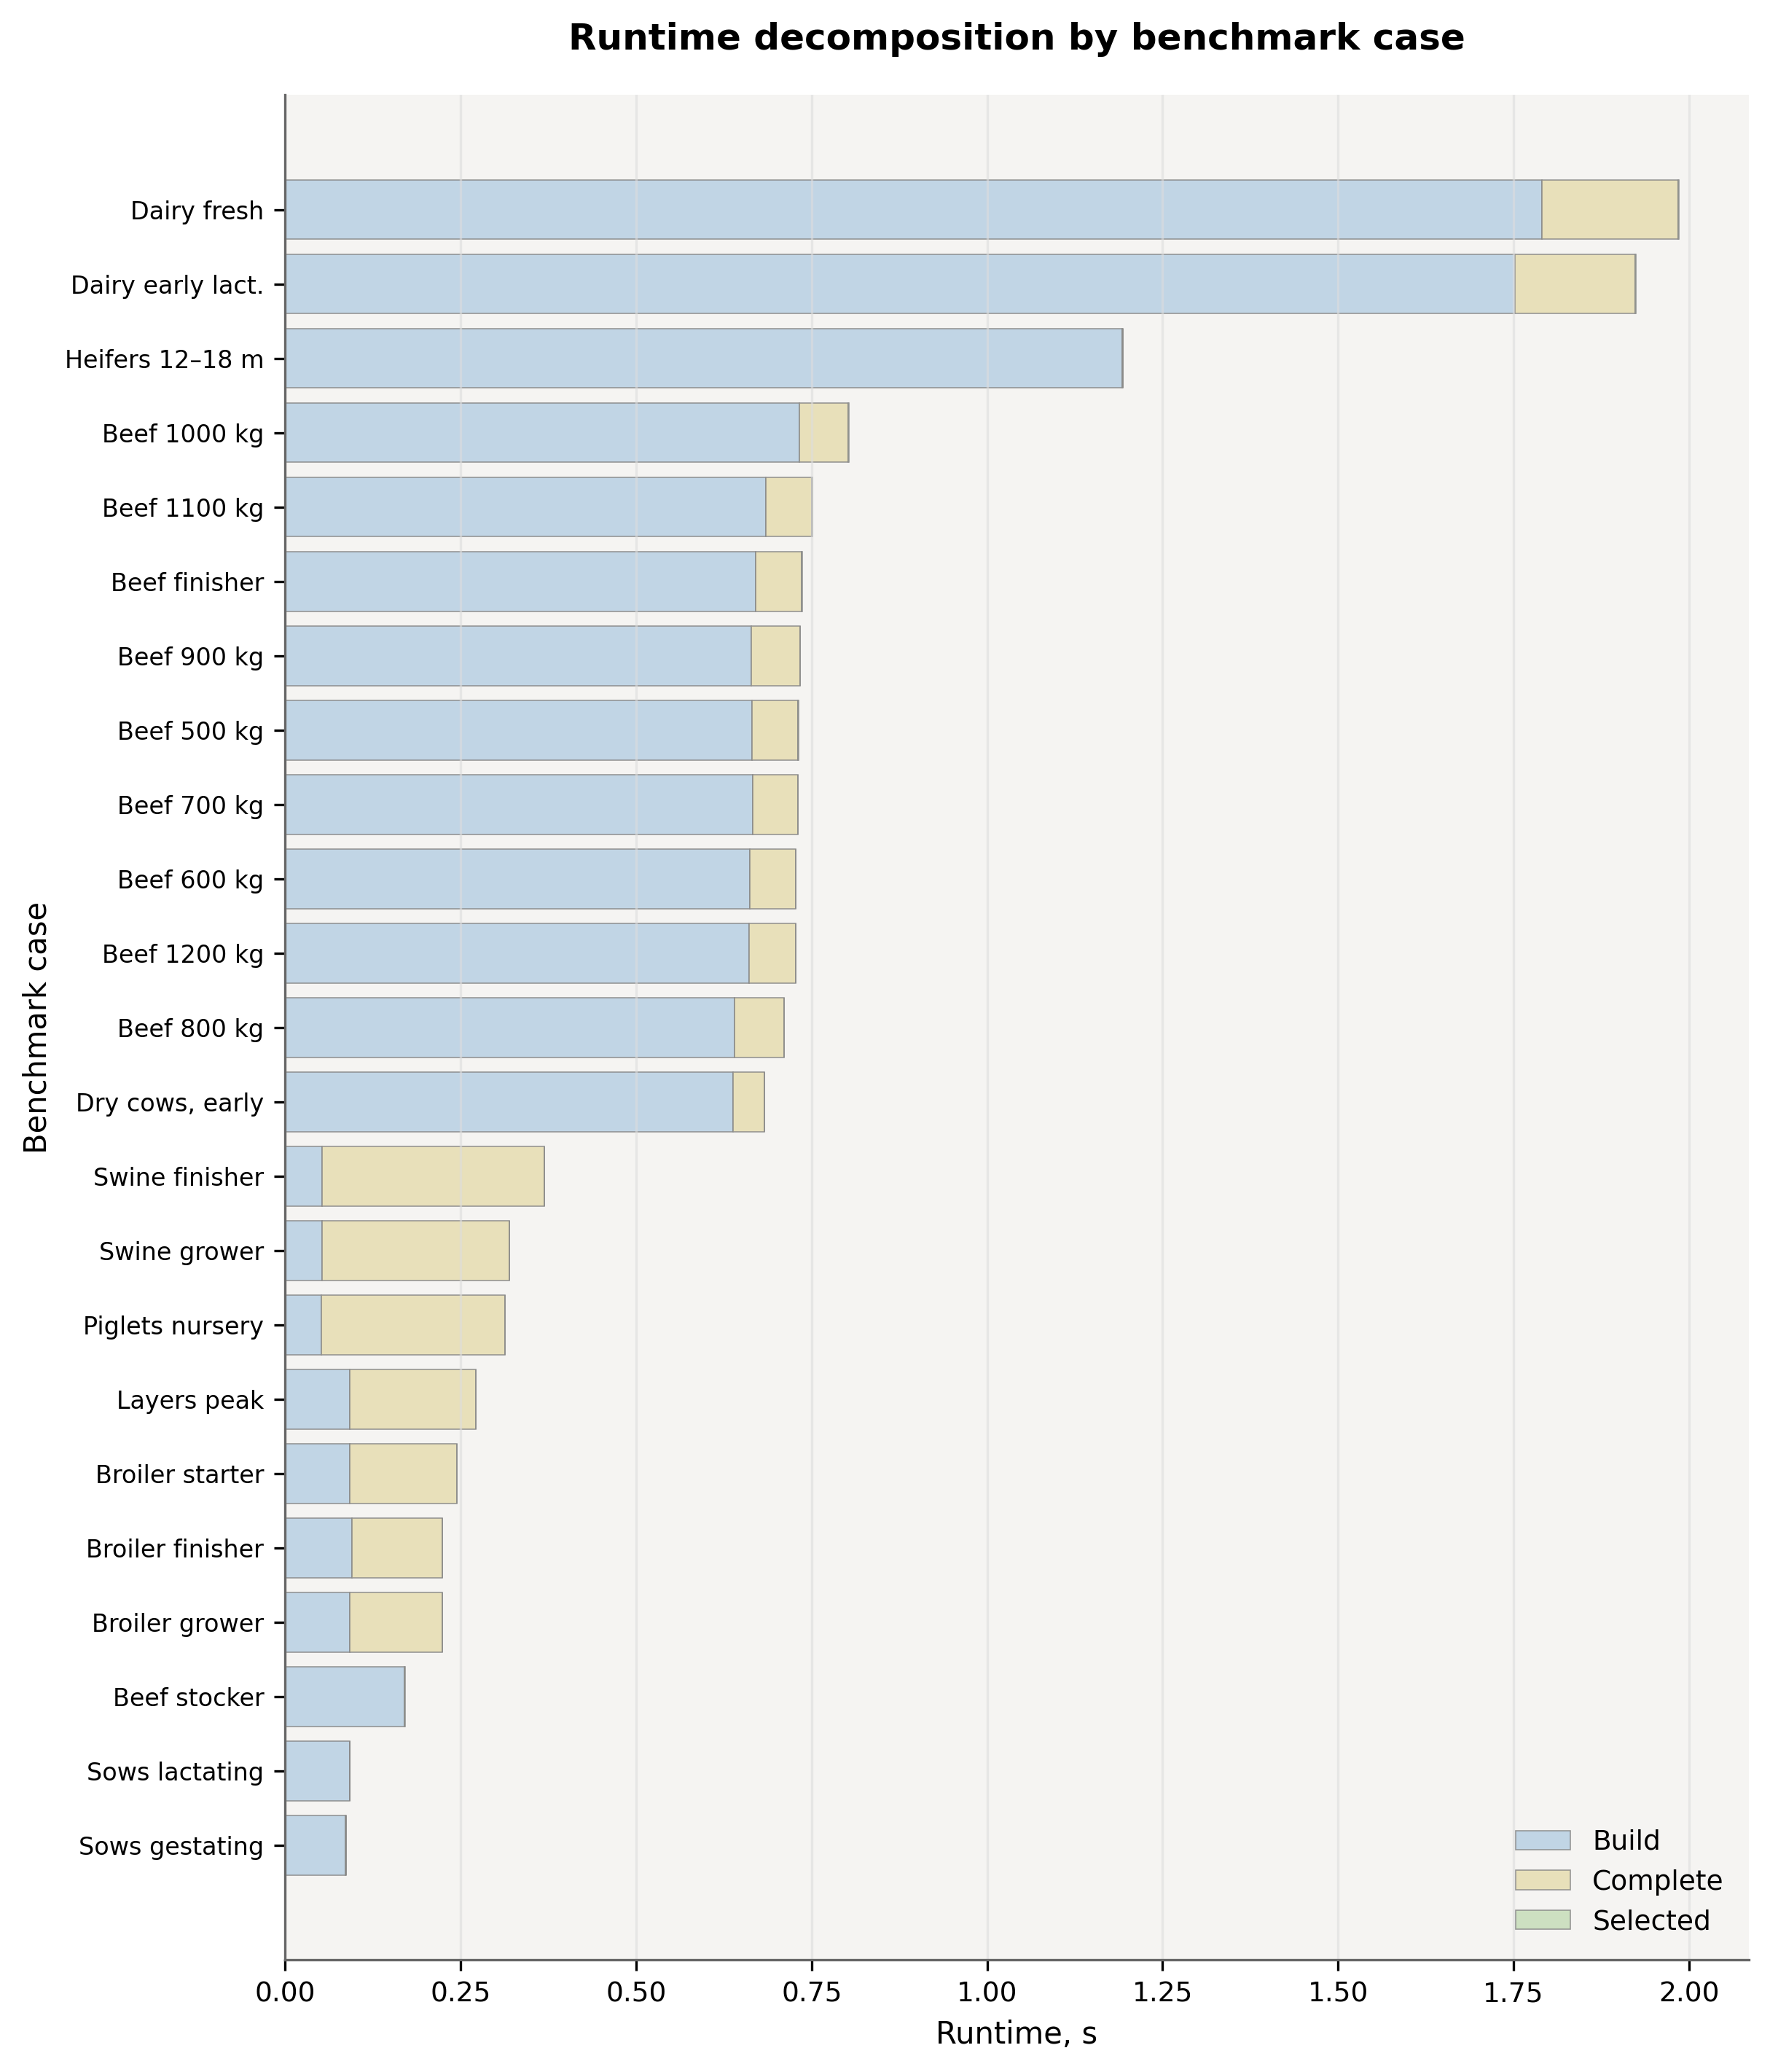
\includegraphics[width=0.88\textwidth]{../manuscript/Figure_4_Runtime.png}
    \caption{Сравнение времени выполнения (Runtime) по рабочим процессам и сценариям. Столбцы демонстрируют относительный вклад каждого режима в общее время вычислений.}
    \label{fig:runtime}
\end{figure}

\subsection{Качество покрытия норм и структура дефицитов}\label{subsec:quality}

Средняя доля выполненных жёстких ограничений составила 64{,}8\%, а средний индекс покрытия норм по всей выборке достиг 81{,}8 из 100.

Влияние предварительного ручного вмешательства на качество рациона продемонстрировано на рисунках~\ref{fig:qualitypoints} и~\ref{fig:qualitydelta}. Процесс \texttt{complete\_from\_library} (покрытие 85{,}0) систематически улучшал качество рациона по сравнению с автоматическим построением с нуля (покрытие 83{,}2), что подчеркивает ценность пользовательского <<каркаса>> (напр., фиксированные объёмы грубых кормов). Дельта качества была наиболее выражена в сценариях для КРС. Процесс \texttt{selected\_only} продемонстрировал наименьшее покрытие (77{,}1) вследствие искусственно суженного набора ингредиентов.

\begin{figure}[htbp]
    \centering
    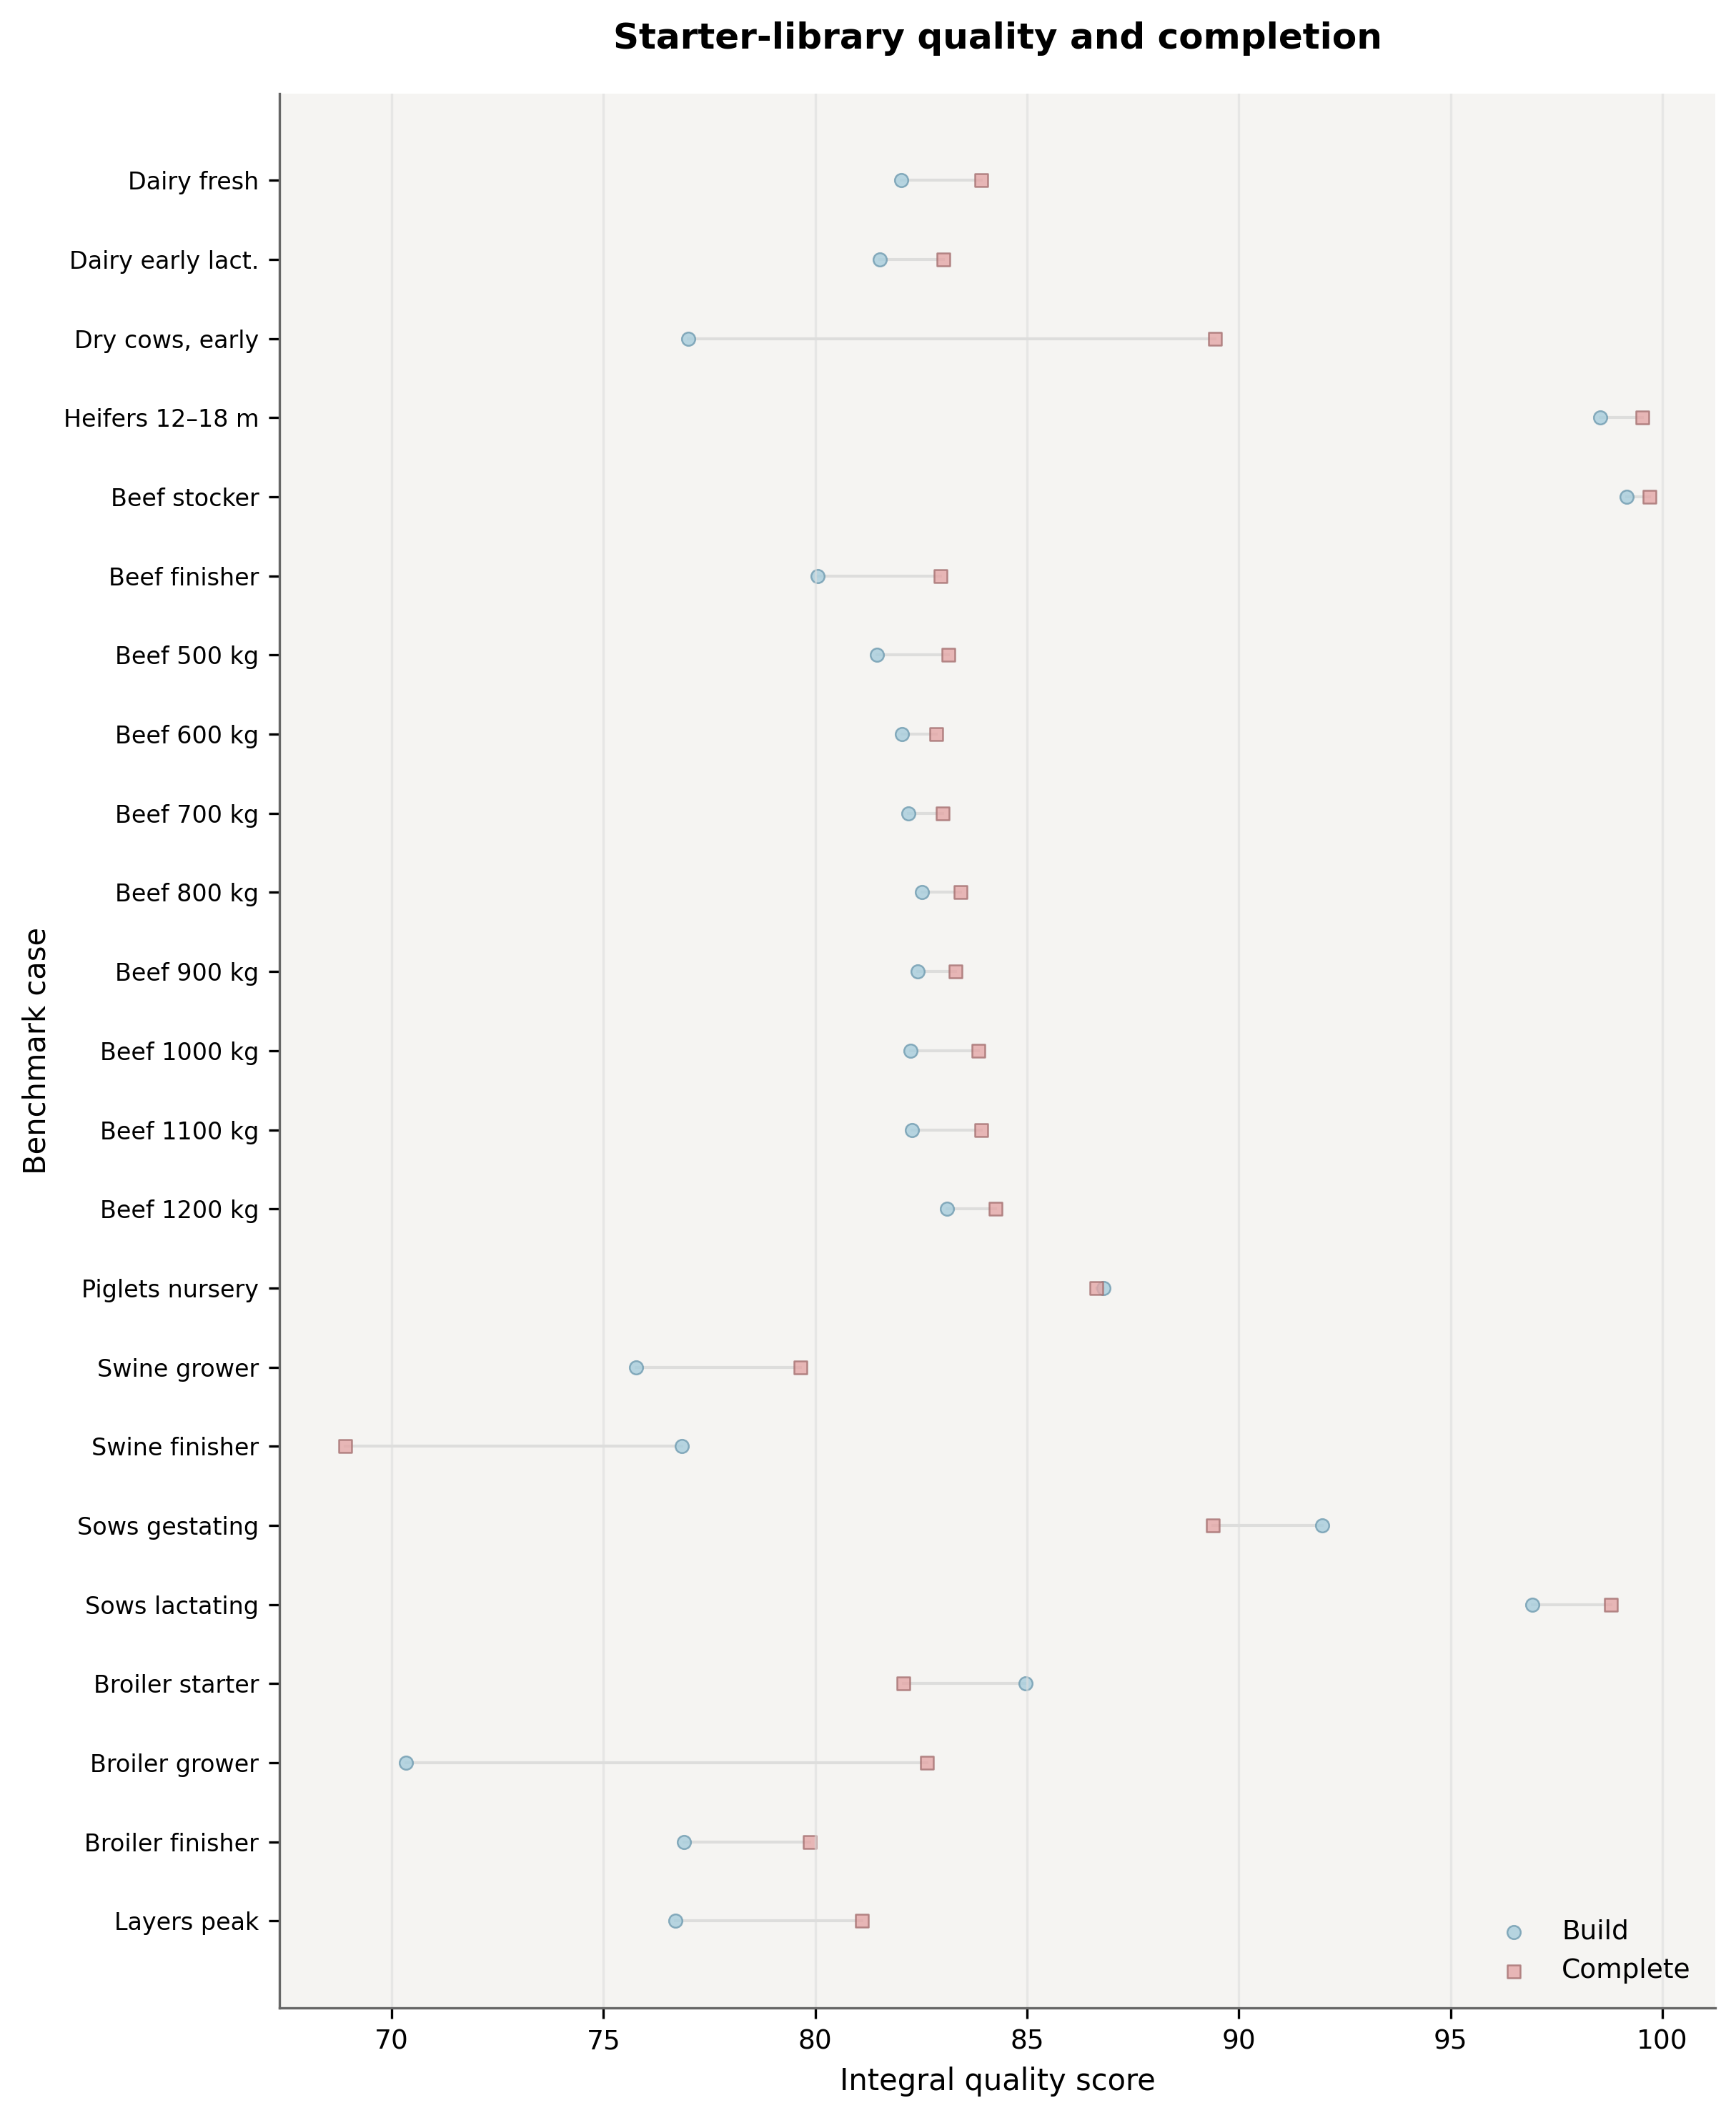
\includegraphics[width=0.85\textwidth]{../manuscript/Figure_2_Quality_Points.png}
    \caption{Сравнение Индекса покрытия норм между режимами \texttt{build\_from\_library} и \texttt{complete\_from\_library}.}
    \label{fig:qualitypoints}
\end{figure}

\begin{figure}[htbp]
    \centering
    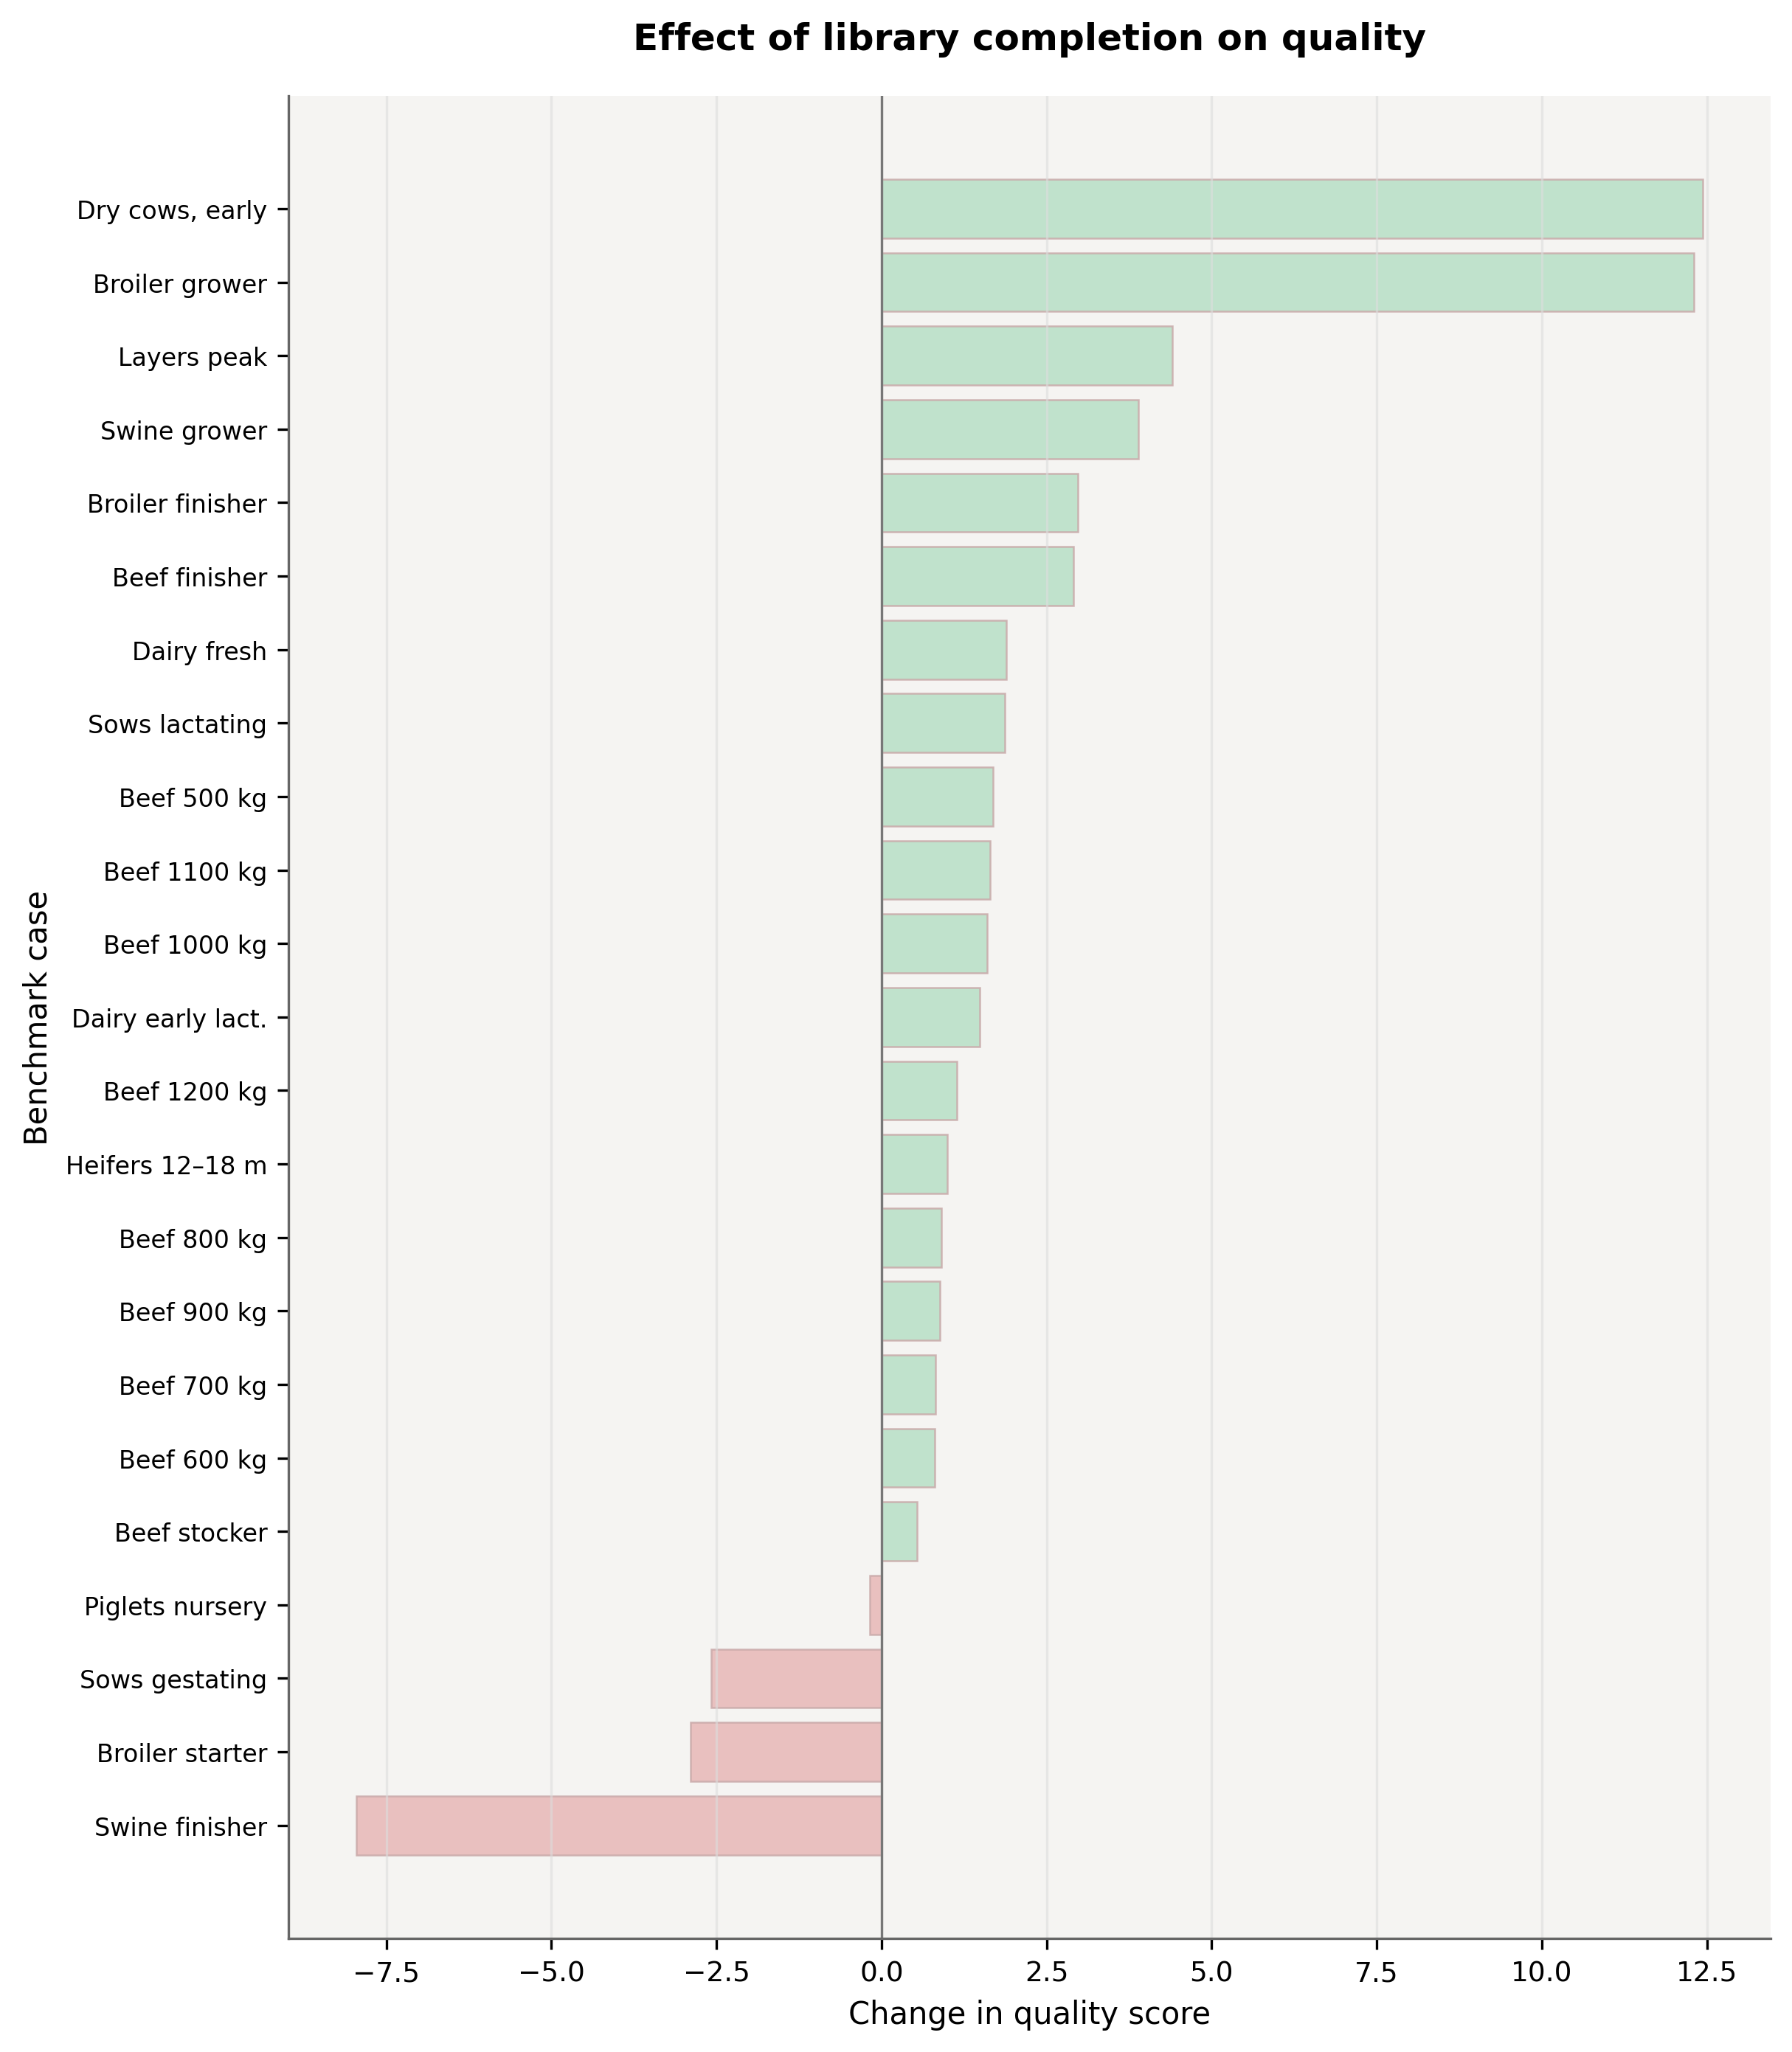
\includegraphics[width=0.85\textwidth]{../manuscript/Figure_3_Quality_Delta.png}
    \caption{Дельта качества (разность индексов покрытия) при переходе от автоматического построения к балансировке пользовательского каркаса рациона.}
    \label{fig:qualitydelta}
\end{figure}

Углублённый анализ систематических дефицитов был проведён для моногастричных животных (свиньи и птица; дополнительные Таблицы~S5, S6). Тепловая карта (Рисунок~\ref{fig:heatmap}) иллюстрирует кумулятивную выраженность отклонений. Основными лимитирующими факторами оставались фосфор, плотность кальция, витамин D3, натрий, лизин или его прокси-ограничения и сумма метионина и цистина в зависимости от вида и стадии.

\begin{figure}[htbp]
    \centering
    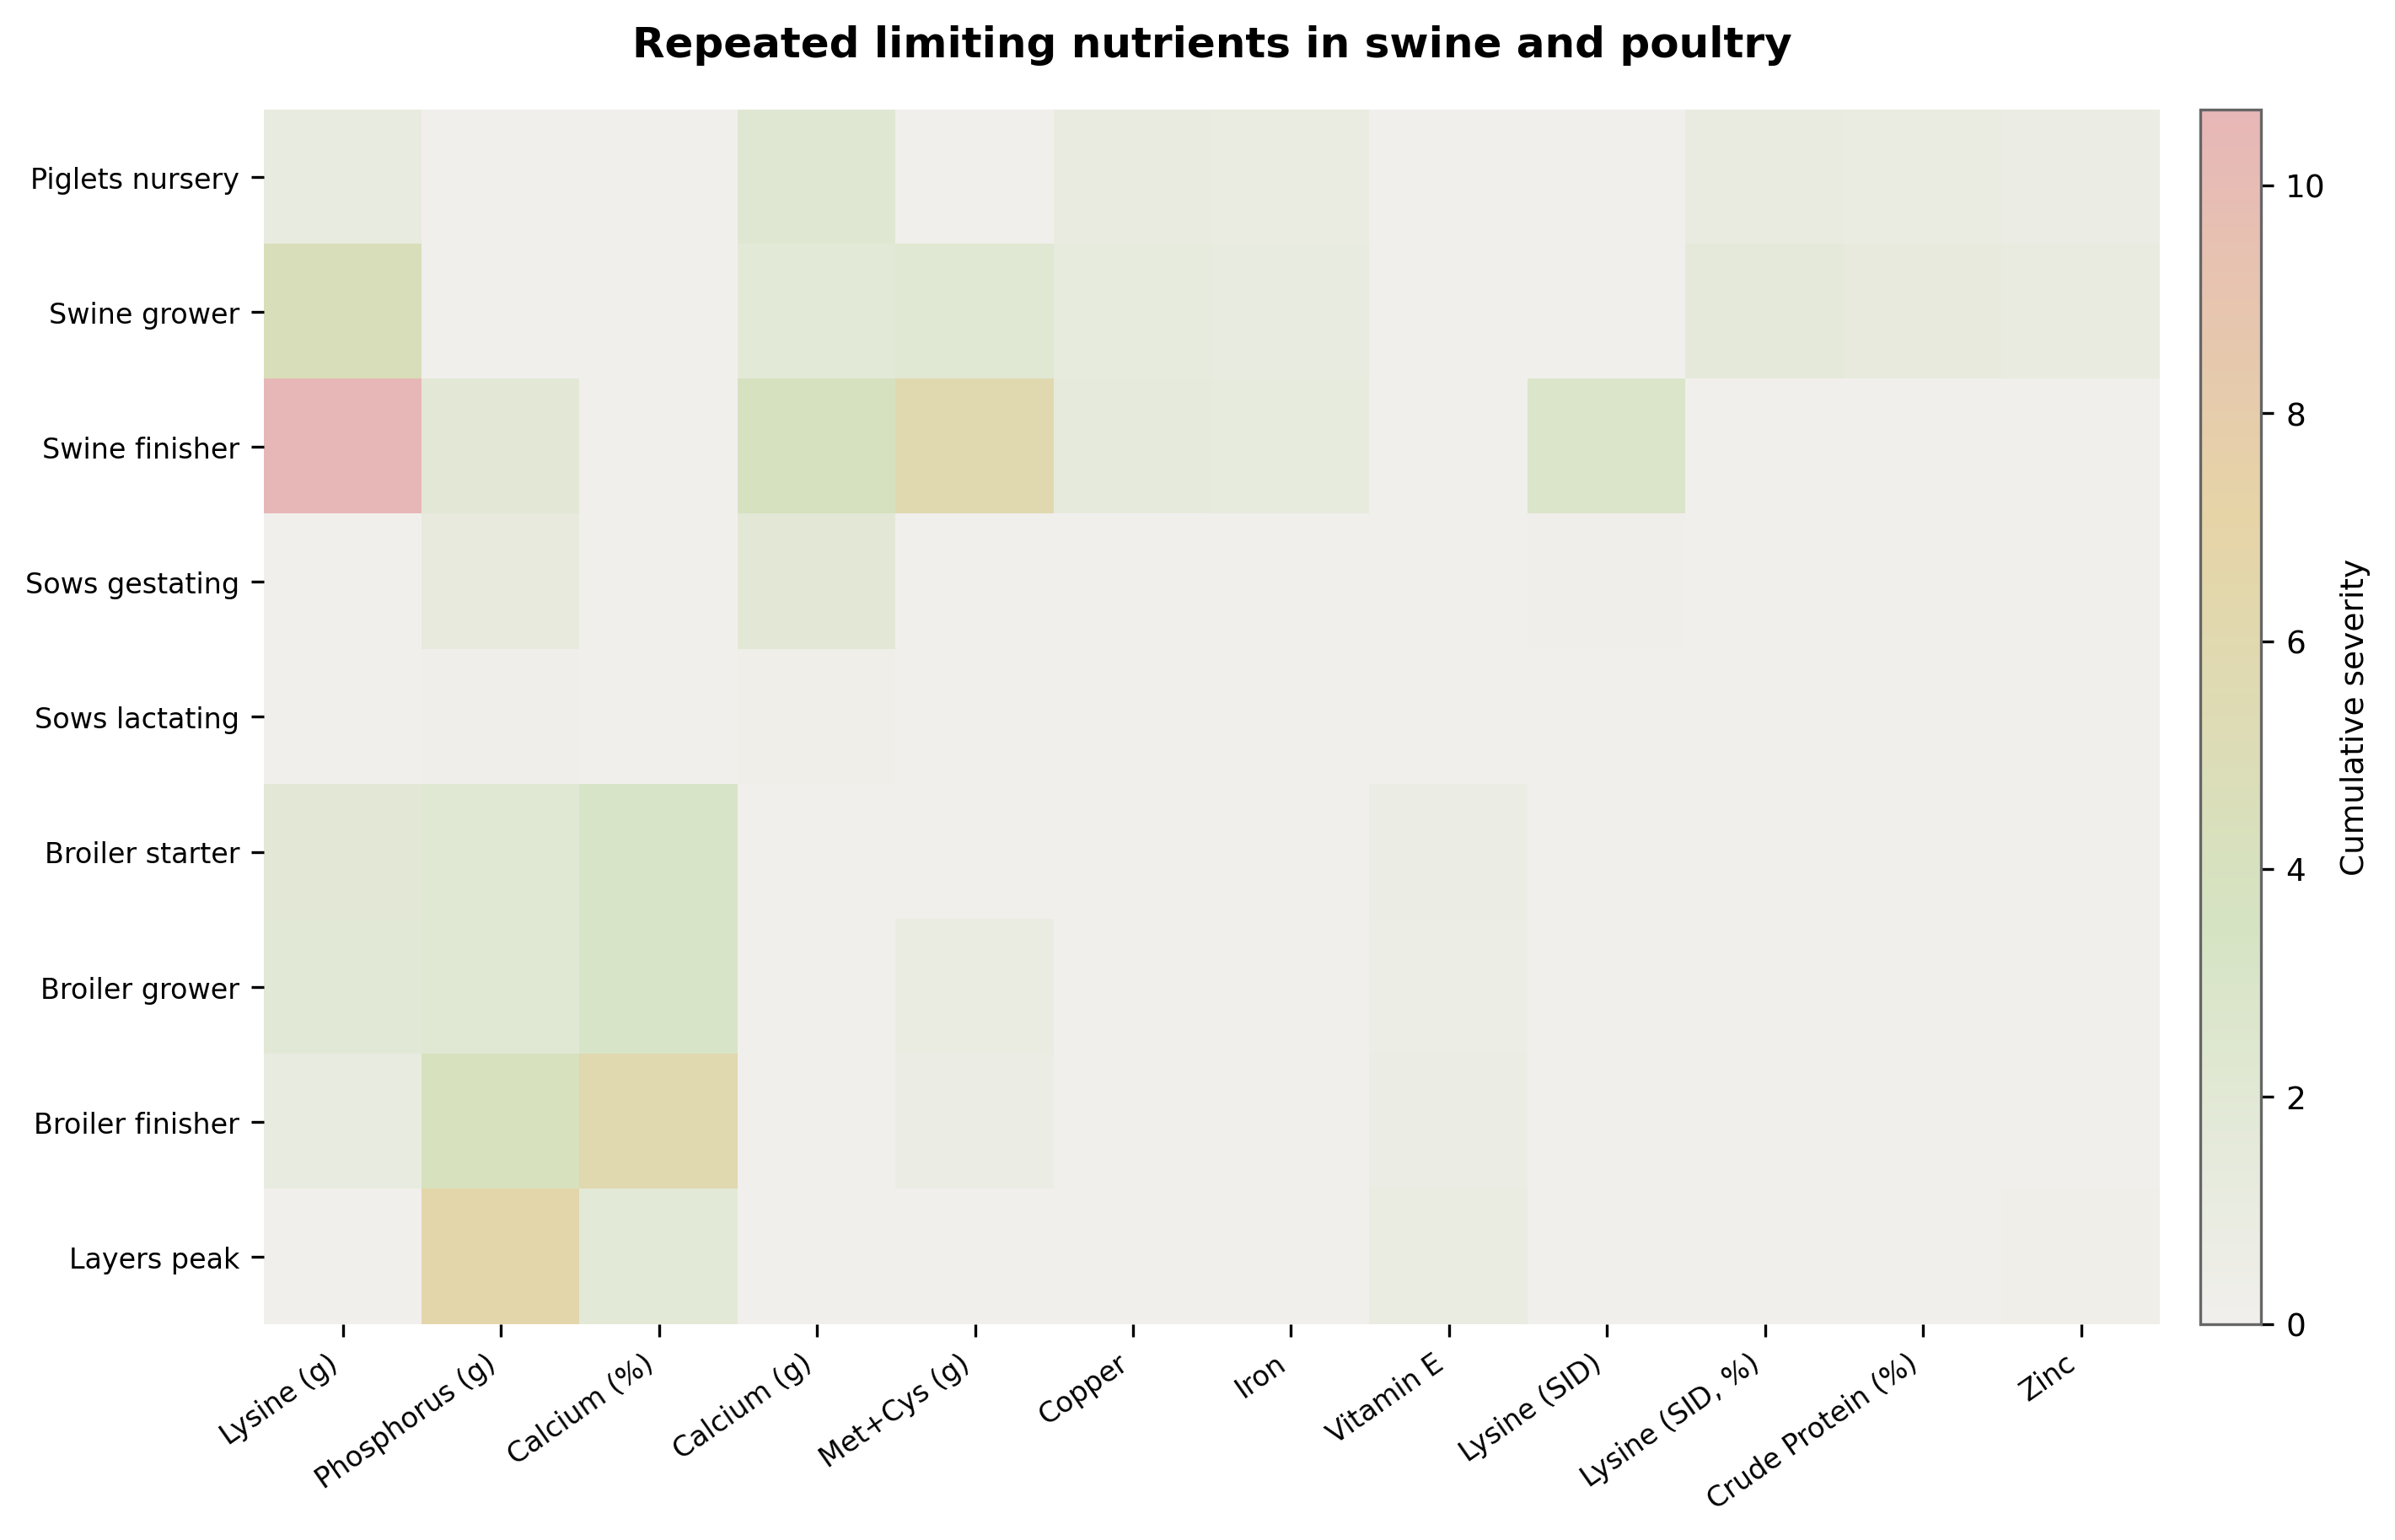
\includegraphics[width=0.92\textwidth]{../manuscript/Figure_5_Heatmap.png}
    \caption{Кумулятивная выраженность дефицитов нутриентов (по величине отклонения от нормы) в завершённых рационах для сценариев свиней и птицы.}
    \label{fig:heatmap}
\end{figure}

\subsection{Экономический анализ и оценка LLM}\label{subsec:economic}

Средняя стоимость рациона составила 183{,}0 руб./сут. Рисунок~\ref{fig:costscatter} демонстрирует нелинейную зависимость между стоимостью и рабочим процессом, формирующую видоспецифичные кластеры. Для КРС два рациона с одинаковым числом ингредиентов могли существенно различаться по стоимости и полезности в зависимости от баланса грубых и концентрированных кормов. Для птицы относительно небольшие добавки нутриентно плотных кормов могли существенно улучшить покрытие норм.

\begin{figure}[htbp]
    \centering
    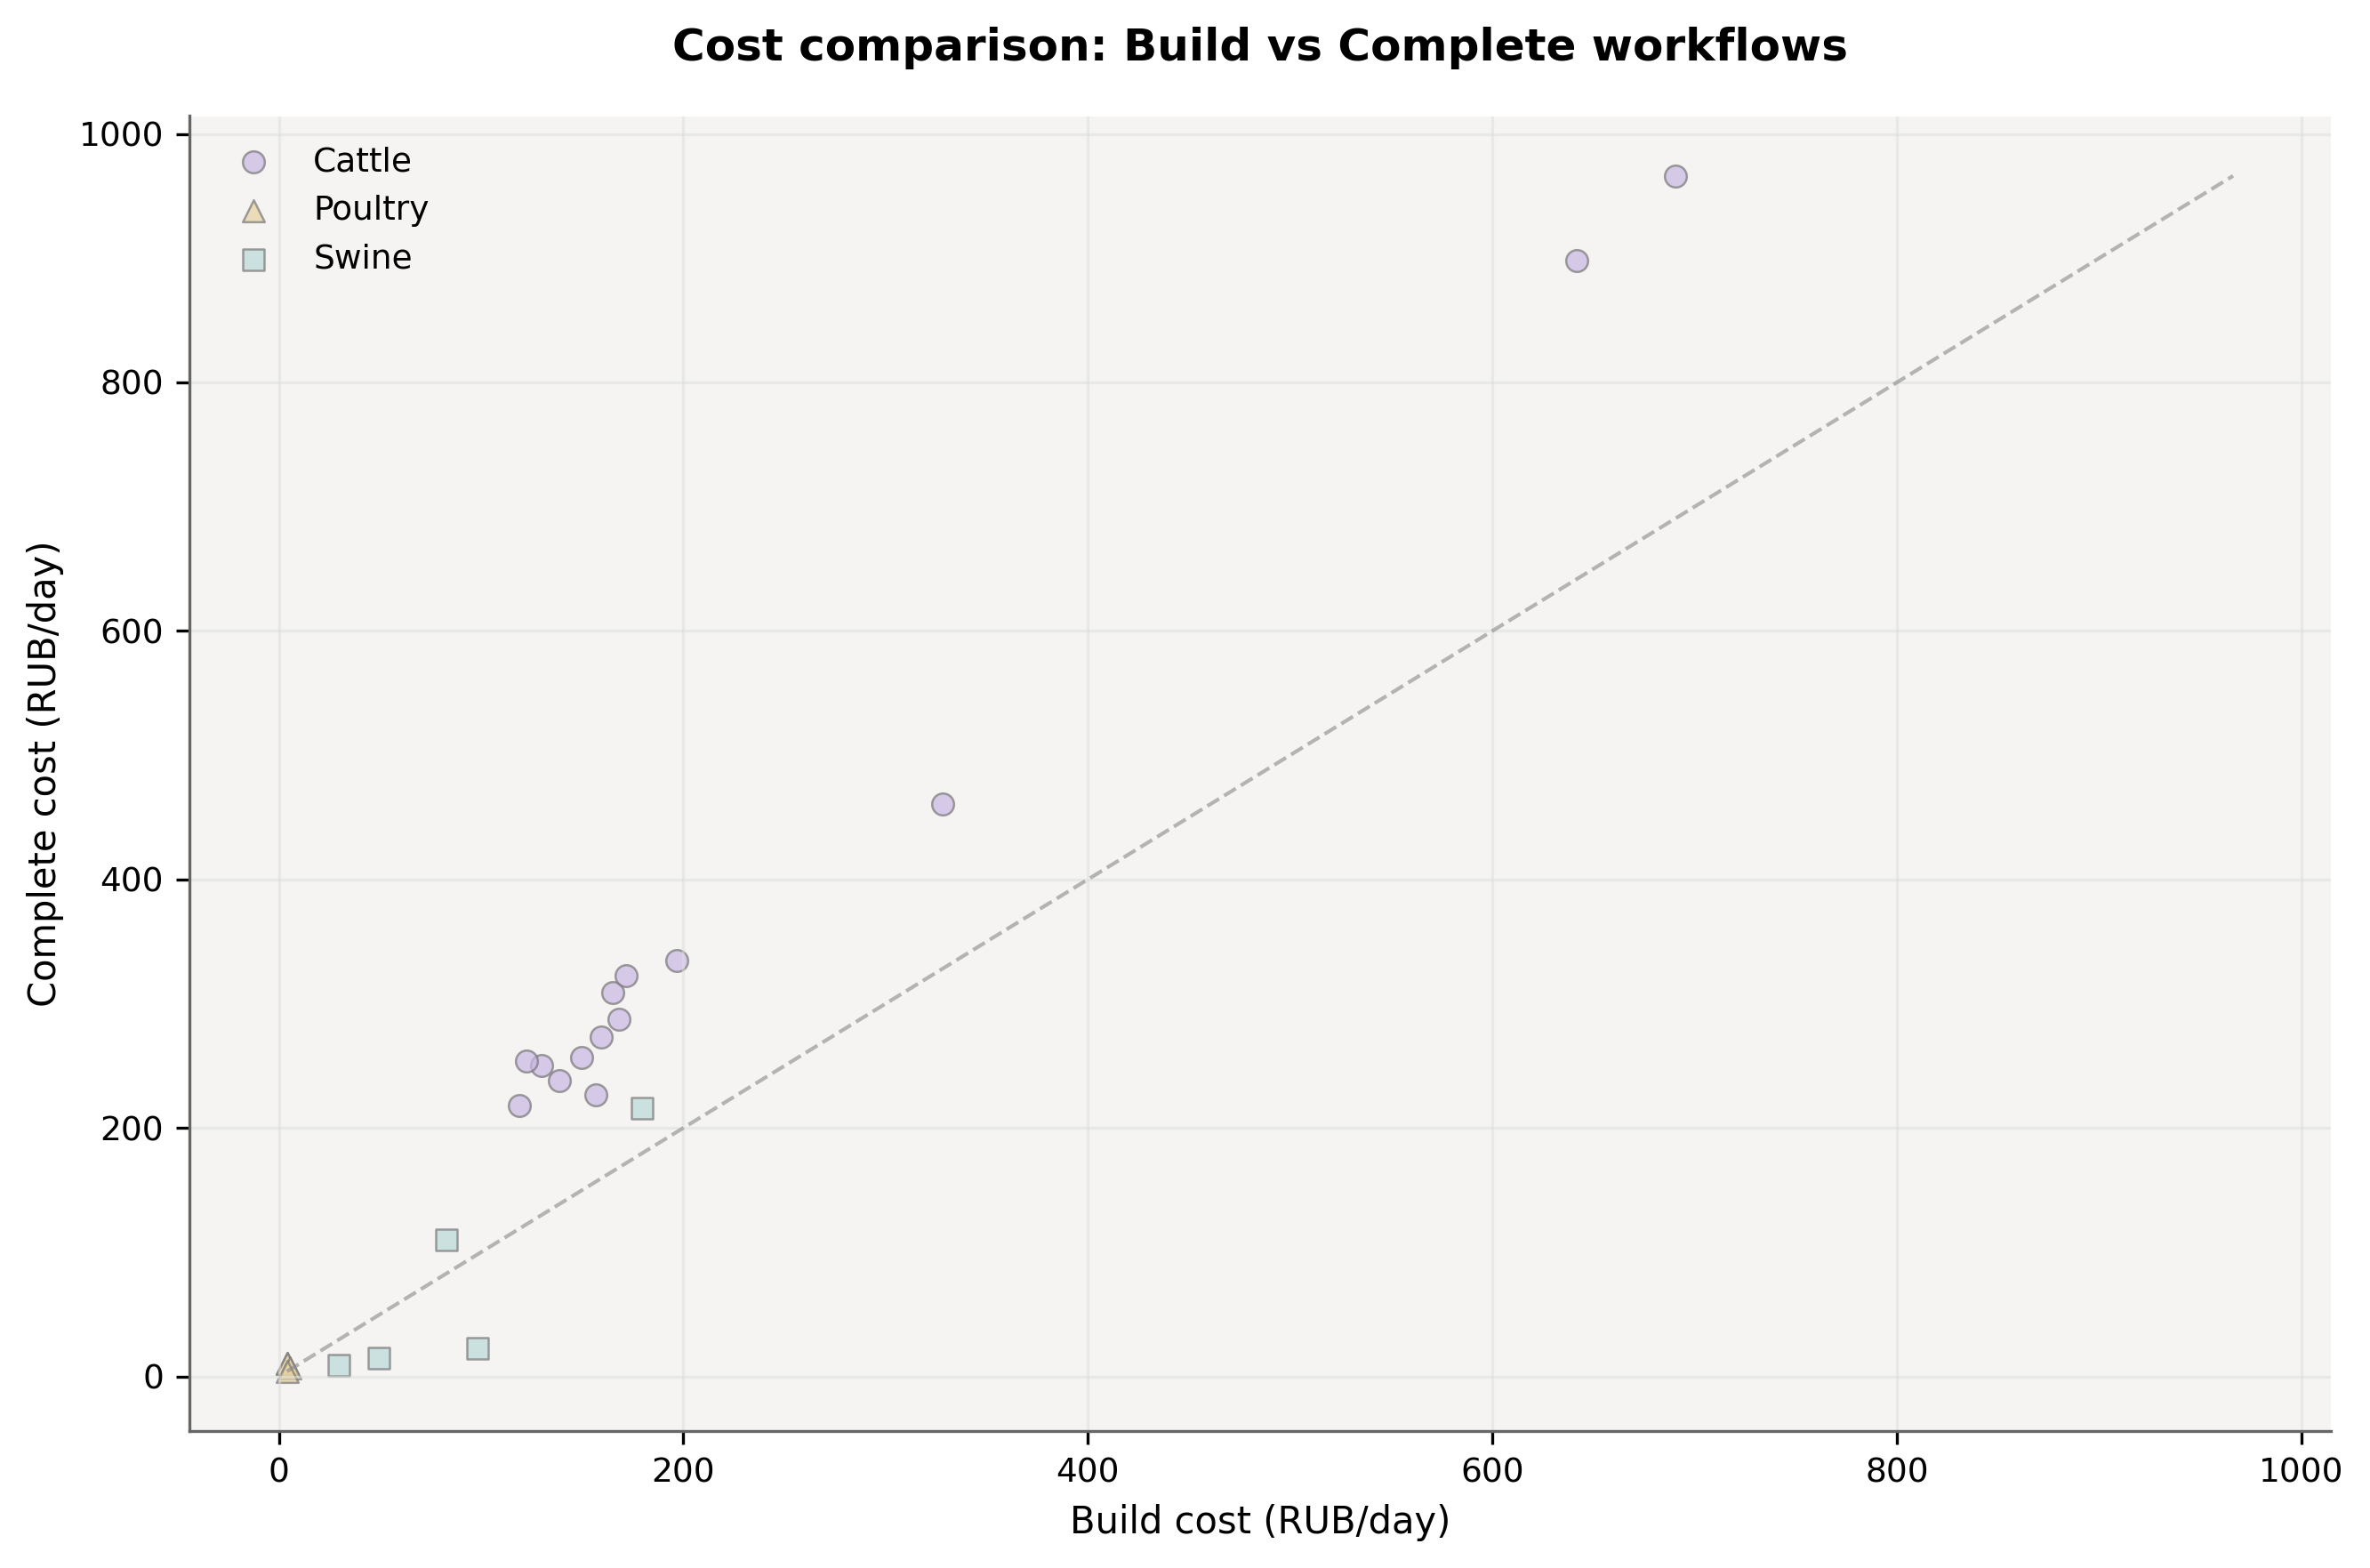
\includegraphics[width=0.82\textwidth]{../manuscript/Figure_6_Cost_Scatter.png}
    \caption{Зависимость стоимости рациона от применяемого режима оптимизации с кластеризацией по видам животных.}
    \label{fig:costscatter}
\end{figure}

Оценка локального консультационного агента по обеим протестированным конфигурациям Qwen (Таблица~\ref{tab:llm-eval}) показала ограниченную полезность. Ни одна из конфигураций не продемонстрировала преимущества перед другой: как настройка 4B/4096, так и 9B/2048 показали recall лимитирующих нутриентов@3 = 0{,}17, обоснованность рекомендаций@3 = 0{,}67, точность lookup = 0{,}50 и общую применимость = 34{,}2/100. Что важно, добавленная benchmark-телеметрия показала, что эти результаты были получены без скрытого fallback по модели или контексту. Таким образом, текущее ограничение объясняется не скрытой деградацией инфраструктуры, а недостаточной производительностью задач в рамках роли ограниченного консультанта.

\begin{table}[htbp]
\caption{Ограниченный benchmark внутриприложенного консультирования для локальных конфигураций Qwen 3.5 на 12 задачах.}\label{tab:llm-eval}
\begin{tabular*}{\tblwidth}{@{}LLLLLL@{}}
\toprule
Конфигурация & Recall лимит.@3 & Обосн. rate@3 & Точность lookup & Общая примен. & Интерпретация \\
\midrule
Qwen 3.5 4B @ 4096 & 0{,}17 & 0{,}67 & 0{,}50 & 34{,}2/100 & Непригоден для надёжного консульт. \\
Qwen 3.5 9B @ 2048 & 0{,}17 & 0{,}67 & 0{,}50 & 34{,}2/100 & Нет улучшения при огранич. контексте \\
\bottomrule
\end{tabular*}
\end{table}

\section{Обсуждение}\label{sec:discussion}

Результаты benchmark подтверждают, что три рабочих процесса Felex следует интерпретировать как различные прикладные режимы работы, а не как эквивалентные настройки одного и того же решателя. Процесс \texttt{selected\_only} чрезвычайно быстр, но структурно ограничен пользовательским набором кормов. Процесс \texttt{build\_from\_library} предлагает наиболее широкий поиск, но даже этот режим оставался субсекундным в среднем в текущем benchmark. Процесс \texttt{complete\_from\_library} обеспечил наилучший баланс в текущем benchmark, сочетая существенно лучшее покрытие норм с временем выполнения, достаточным для рутинного использования специалистом. Для прикладной аудитории животноводов это наиболее значимый результат: Felex работает лучше всего, когда расширяет экспертный каркас рациона, а не когда от него требуется полностью заменить экспертный вклад.

Такое позиционирование согласуется и с текущим программным ландшафтом. Felex не является заменой корпоративных формуляционных комплексов или интегрированных платформ управления хозяйством \citep{datacor2026, korall2026, onecow2026}. Его более обоснованная ниша~--- локальный прозрачный инструмент для специалистов, которым необходимы явные рабочие процессы, поддержка нескольких нормативных контуров и снижение зависимости от закрытых облачных экосистем. Эта ниша особенно актуальна в российских условиях, где локализованные инструменты существуют \citep{deltakorm2026, winmix2026}, но открытые, протестированные, локально развертываемые альтернативы остаются ограниченными.

Нутриентное поведение текущего движка согласуется с практической логикой формуляции. Для КРС учёт обменной энергии остаётся прагматичным компромиссом для межвидового инструмента \citep{inra2018, volden2011, kalashnikov2003}. Для моногастричных животных рекуррентное давление в области переваримости аминокислотных ограничений и фосфора подтверждает продолжающуюся важность формуляции с учётом переваримости \citep{stein2007, nRC2012, pomar2021, deLange2012, vanmilgen2015}. Наблюдаемая доля выполнения жёстких ограничений около 65\% не должна интерпретироваться как простой алгоритмический провал; она также отражает несовершенство данных о кормах, разреженность ценовых якорей и биологическую сложность одновременного удовлетворения всех уровней из ограниченной библиотеки. Нутриентный контур, матрица структурных ограничений кормов и категориальный состав нормализованной кормовой базы, используемые для интерпретации этих закономерностей, документированы соответственно в дополнительных Таблицах~S7, S8 и S9. Иерархическая LP-стратегия и fallback-шаг с мягкими целями остаются обоснованными для практического построения рационов в данных условиях \citep{rehman1987}.

Результаты локального агента требуют более осторожной интерпретации, чем предполагалось в предыдущей версии рукописи. В рамках ограниченного benchmark внутриприложенного консультирования обе протестированные конфигурации Qwen показали одинаково низкий агрегированный балл адекватности, и более крупная модель 9B не улучшила результат 4B при ограниченном контекстном окне. Поскольку benchmark-телеметрия не зафиксировала скрытого fallback по модели или контексту, эти слабые результаты объясняются производительностью задач, а не скрытой деградацией инфраструктуры. На текущем этапе агент лучше всего характеризуется как экспериментальный пояснительный слой, способный иногда обобщать, контекстуализировать и предлагать кандидатные корректировки, оставляя ответственность за интерпретацию за специалистом.

Ряд ограничений вытекает непосредственно из состояния репозитория и benchmark-данных. Во-первых, оптимизационное ядро остаётся линейным, тогда как нелинейные, многокритериальные, стохастические и эволюционные подходы могут лучше отражать некоторые биологические компромиссы и неопределённость состава \citep{li2022nonlinear, uyeh2018, uyeh2019, das2023, agrawal2025, kumar2025}. Во-вторых, региональную кормовую базу необходимо расширять и непрерывно курировать; текущий benchmark-ready каталог полезен, но опирается на ограниченное число прямых ценовых якорей. В-третьих, нормативный движок должен быть дополнен более богатыми факториальными производными, особенно для региональной практики, стадийно-специфичных производственных состояний и анализа чувствительности с учётом неопределённости. В-четвёртых, локальный агентный слой не следует расширять только путём масштабирования модели: в текущем ограниченном benchmark более крупная модель при меньшем контекстном окне не улучшила адекватность. Будущие работы должны сочетать улучшенные региональные данные о кормах, более богатый вывод норм, анализ неопределённости, отслеживаемые рекомендации и, для агентного слоя, лучшую привязку к задачам и доменную адаптацию вместо простого увеличения параметров.

\section{Заключение}\label{sec:conclusion}

Felex демонстрирует, что локально развертываемая платформа для расчёта рационов может сочетать прозрачные оптимизационные рабочие процессы, поддержку нескольких нормативных контуров и практичную настольную среду выполнения без привязки к cloud-first архитектуре. В текущем состоянии наиболее убедительным сценарием применения остаётся вспомогательное построение рационов для специалистов малых хозяйств и животноводческого бизнеса, особенно там, где важны региональная адаптация и операционная автономность. Настоящий benchmark подтверждает это практическое позиционирование, одновременно демонстрируя явные ограничения в покрытии кормовой базы, обработке неопределённости и пригодности локального агента для надёжного консультирования. Эти ограничения определяют повестку дальнейшего развития более чётко, чем любые заявления о зрелости автоматизации.

% Author contributions (CRediT taxonomy) - printed via \printcredits before references

% Conflict of Interest
\section*{Заявление о конфликте интересов}

Авторы заявляют, что не имеют известных конкурирующих финансовых интересов или личных отношений, которые могли бы повлиять на работу, представленную в данной статье.

% Funding
\section*{Финансирование}

Исследование выполнено без внешнего финансирования.

% Data Availability
\section*{Заявление о доступности данных}

Исходный код системы Felex доступен по адресу \url{https://github.com/danilkotelnikov/Felex}. Канонический оптимизационный benchmark-артефакт хранится по адресу \url{https://github.com/danilkotelnikov/Felex/tree/main/.claude/benchmarks}, основной JSON~--- \url{https://github.com/danilkotelnikov/Felex/blob/main/.claude/benchmarks/results/benchmark_results.json}. Артефакты ограниченного агентного benchmark хранятся по адресам \url{https://github.com/danilkotelnikov/Felex/tree/main/deliverables/agent_publication_benchmark_2026-04-03_qwen4b_4096} и \url{https://github.com/danilkotelnikov/Felex/tree/main/deliverables/agent_publication_benchmark_2026-04-03_qwen9b_2048}. Нормализованный экспорт кормовой базы доступен по адресу \url{https://github.com/danilkotelnikov/Felex/blob/main/database/output/feeds_database.json}. Дополнительные данные и скрипты предоставляются автором для корреспонденции по обоснованному запросу.

% Acknowledgments
\section*{Благодарности}

Авторы выражают благодарность разработчикам библиотеки \texttt{good\_lp}, экосистемы Ollama и создателям открытых сельскохозяйственных стандартов и справочных ресурсов, сделавших данную работу возможной.

% AI Use Declaration
\section*{Заявление об использовании генеративного ИИ и технологий на основе ИИ при подготовке рукописи}

При подготовке данной работы авторы использовали \textbf{Anthropic Claude} (Claude Opus 4.6 и Claude Sonnet, \url{https://www.anthropic.com/claude}) и \textbf{OpenAI Codex} (\url{https://openai.com/index/openai-codex/}) для помощи в синтезе литературы, рецензировании документации кода, языковому редактированию рукописи, форматированию LaTeX и аудиту benchmark-документации. После использования этих инструментов авторы проверили и отредактировали содержание по мере необходимости и несут полную ответственность за содержание опубликованной статьи.

% Print CRediT authorship contributions
\printcredits

% Bibliography
\bibliographystyle{cas-model2-names}
\bibliography{../manuscript/felex_references}

\end{document}
